\documentclass[10pt,
%handout
]{beamer}
\usepackage[utf8]{inputenc}
\usepackage[T1]{fontenc}
\usepackage{lmodern}

\usepackage{nicefrac}
\usepackage{braket}

%\usepackage[backend=biber,style=chem-acs]{biblatex}
%\bibliography{biblio}


\usetheme{metropolis}
\setbeamercolor{block title}{use=structure,fg=white,bg=structure.fg!75!black}
\setbeamercolor{block body}{parent=normal text,use=block title,bg=block title.bg!10!bg}


\usepackage{tikz}
\usetikzlibrary{positioning, decorations.markings, decorations.pathmorphing, calc}

\usepackage{siunitx}
\usepackage{mhchem}
\usepackage{minted}

\author{Pierre Beaujean (\href{mailto:pierre.beaujean@unamur.be}{pierre.beaujean@unamur.be})}
\title{Advanced Python for advanced users}
\subtitle{... And a few concepts of computer science}
\institute{University of Namur}
\date{March 2025 (version of  \today)}

\allowdisplaybreaks

\begin{document}
\begin{frame}[plain]
	\maketitle
\end{frame}

\begin{frame}{Table of content}
	\tableofcontents
\end{frame}

\section{Back to basics}

\begin{frame}{Computer?}
	As far as you are concerned, a computer contains:\begin{itemize}
		\item A \textbf{CPU}, which execute (\textit{assembler}) code. Nowadays, there are also \textbf{GPUs} which can fulfill this role.
		\item Different kind of \textbf{memories} (cache, RAM, disk, etc), some of which can be addressed differently (\textit{e.g.}, through files).
		\item Some interfaces to the outside world, via peripherics (screen,  mouse, Ethernet, etc).
	\end{itemize}
	
	By itself, the CPU only moves bytes around in memory, and can perform operation on them. It understands the concept of \textbf{integers} and \textbf{floating point numbers} (IEEE-754 shenanigans), but that's about it. 
	
	Most functionalities of a computer (\textit{e.g.}, files) are in fact available thanks to the \textbf{operating system}, which offers, \textit{e.g.}, an unified interface to peripherics.
\end{frame}

\begin{frame}
	The \textbf{assembler} is a pretty simple (and CPU-dependent) language. For example, it does not understand the concept of strings (which explains why Fortran and C implements them differently). And, among other things, \textit{advanced} concepts like \textit{loops} are not directly available.
	
	 So... A meme will now ensue.
	
	\begin{center}
		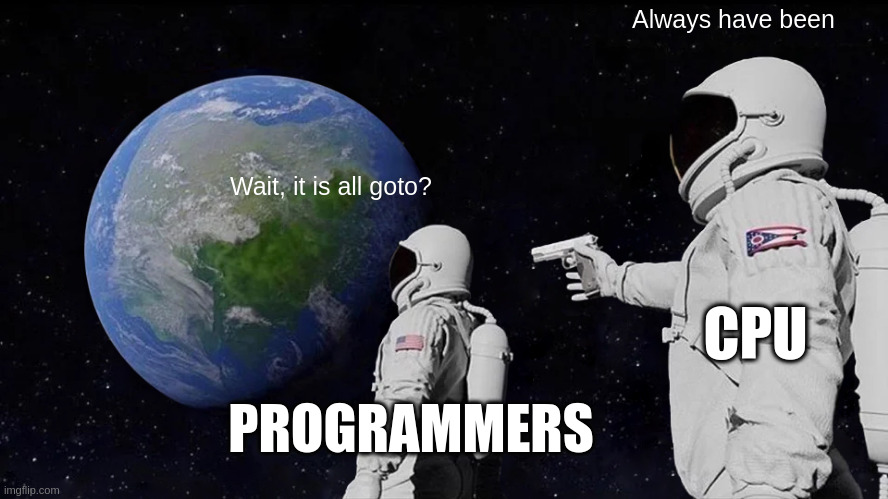
\includegraphics[width=.7\linewidth]{im/meme-goto}
		
		(Note: it is in fact \textbf{conditional jumps})
	\end{center}
\end{frame}

\begin{frame}{Programming}
	The role of a programming language is to allow you to express complex things (\textit{e.g.}, loops) in a ``simple" and readable form, which will be turned into an executable (\textit{i.e.}, a bunch of assemblers) by a \textbf{compiler}, or executed by an \textbf{interpreter}. While the latter is slower, it allows, \textit{e.g.}, for some reflexivity or the capacity to rewrite itself.
	
	Python is an interpreted language. However, much like Java, it is in practice compiled \textit{on the fly} into an intermediate bytecode representation (the content of \texttt{\_\_pycache\_\_}), which in fact improves itself over time (the more you execute the code, the faster it gets, since it deactivates some of the checks).
\end{frame}

\begin{frame}[fragile]
	The way to write the code is referred to as a \textbf{programming paradigm}, a relatively high-level way to conceptualize and structure the implementation of a computer program.\footnote{\url{https://en.wikipedia.org/wiki/Programming_paradigm}} Among others, there are:\begin{itemize}
		\item \textbf{Imperative}, in which the code directly controls execution flow and state change. This includes the famous \textbf{procedural} (\mintinline{text}|x = a(); y = b(x);|) and \textbf{object-oriented} (\mintinline{text}|x = X(); x.b();|) approaches.
		\item \textbf{Declarative}, in which code declares properties of the desired result, but not how to compute it, it describes what computation should be performed. This include the (in)famous \textbf{functional} approach (\mintinline{text}|(b(a()))|), but also programs based on \textbf{logic and constraints}.
		\item \textbf{Concurrent}, \textbf{visual}, etc...
	\end{itemize}
	
	To a certain extent, all paradigm can be used in all languages. Python is generally approached as an POO language.
	\vspace{1em}
\end{frame}

\begin{frame}{Note on the ``who''}
	In this presentation, I will distinguish three kinds of people:\begin{enumerate}
		\item The \textbf{developers}, who actually develop the code/library and eventually provide an API (\textit{application programming interface}).
		\item The \textbf{programmers}, who use the API provided by the code/library and develop on top of it.
		\item The \textbf{users}, who use the program/executable, but do not program.
	\end{enumerate}
\end{frame}

\section{General concepts for programming}

\begin{frame}{Abstractions}
\end{frame}

\begin{frame}{Data structures}
\end{frame}

\begin{frame}{Design by contract}
\end{frame}

\begin{frame}{Documentation}
\end{frame}

\begin{frame}{Testing}
\end{frame}

\begin{frame}{Error handling (\textit{exceptions})}
	content...
\end{frame}

 \section{POO and POO in Python}
 
 \begin{frame}{What is POO?}
 \end{frame}
 
 \section{Organization of a Python project}
 
 \begin{frame}
 	\begin{itemize}
 		\item Don't reinvent the wheel (\textit{battery (already) included})
 		\item README \& LICENSE
 		\item packages (\texttt{import stuff})
 		\item Project (\texttt{pyproject.toml})
 		\item virtualenv
 	\end{itemize}
 \end{frame}

\end{document}